\subsubsection{Job Creation Page Specifications}
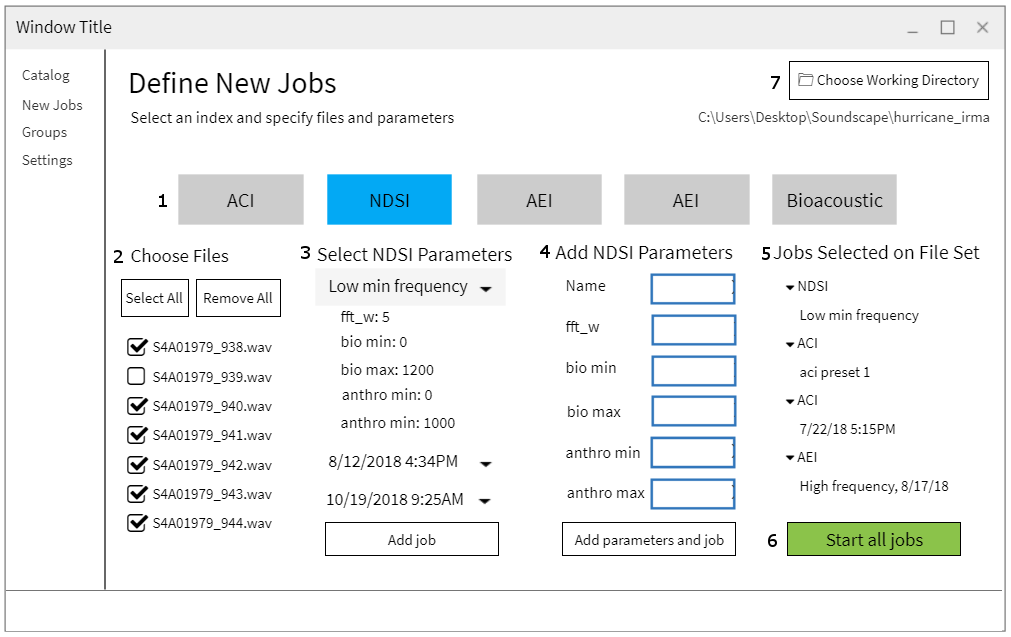
\includegraphics[width=\textwidth]{JobsPage}\\
The jobs page is where the user will select parameters and inputs, and queue jobs to be processed either on their local machine, or on their server where they have the server application running. These jobs and their outputs are then stored in the local database, again either on the local machine or the server, if that is how the user is running the service. The functionality is as follows:\\
\begin{enumerate}
    \item \textbf{Job Index Selection}\\ Each job must have an index to run on the selected inputs. These indices each calculate different data on the input files and are left to the user\textquotesingle s discretion.
    \item \textbf{Input File Selection}\\ This area is populated with related sound files in the current work directory. The user can then selected any of those files they wish to run analysis on. More information on the working directory is found in item 7.
    \item \textbf{Saved Index Parameter Selection}\\ The user has the capability of adding custom preset index/parameter pairs. If the user uses the same index and parameters often, it is useful for them to be able to easily select those options. Any custom saved index/parameter pairs will show here for the user to select. When selected, the user can press the "Add job" button to run the saved index/parameter set on the selected inputs.
    \item \textbf{New Index Parameter Selection}\\ Alternatively, if the user wishes to provide new parameters for the selected index, they can do so here. After selecting the "Add parameters and job" button, the selected index/parameter set will be saved, and the user can either name it for further use, or opt not to, where it will then be named the date and time of creation. Then the service will run the new index/parameter set on the selected inputs.
    \item \textbf{Job Specifications}\\ Here the current set of jobs that the user has defined on the input set are shown. The name of the index and the chosen parameters are shown for each specified job. The user can remove any of these jobs at their discretion.
    \item \textbf{Start All Jobs}\\ As the user creates jobs on selected inputs, they will be added to a queue. When the user is ready, they will select this button to run the chosen jobs in item 5 on the selected inputs in item 2.
    \item \textbf{Working Directory}\\ The working directory is where the service will look for chosen input files. This is an important aspect of the service, as the user may be working on a server where sound files are frequently moved. The user can specify where they would like to grab sound files from whenever they want, without having to worry about files being moved. If files are moved, the service will return an error stating that the file could not be found, and to change the working directory as needed.
\end{enumerate}